\documentclass[11pt,a4paper]{article}

\usepackage[margin=1in, paperwidth=8.3in, paperheight=11.7in]{geometry}
\usepackage{amsfonts}
\usepackage{amsmath}
\usepackage{amssymb} 
\usepackage{enumerate}
\usepackage{enumitem}
\usepackage{fancyhdr}
\usepackage{graphicx}
\usepackage{hyperref}

\begin{document}

\pagestyle{fancy}
\setlength\parindent{0pt}
\allowdisplaybreaks

\renewcommand{\headrulewidth}{0pt}

% Cover page title
\title{Machine Learning - Notes}
\author{Dom Hutchinson}
\date{\today}
\maketitle

% Header
\fancyhead[L]{Dom Hutchinson}
\fancyhead[C]{Machine Learning - Notes}
\fancyhead[R]{\today}

% Counters
\newcounter{definition}[section]
\newcounter{example}[section]
\newcounter{notation}[section]
\newcounter{remark}[section]
\newcounter{theorem}[section]
\newcounter{proof}[section]

% commands
\newcommand{\dotprod}[0]{\boldsymbol{\cdot}}
\newcommand{\cosech}[0]{\mathrm{cosech}\ }
\newcommand{\cosec}[0]{\mathrm{cosec}\ }
\newcommand{\sech}[0]{\mathrm{sech}\ }
\newcommand{\blocks}[0]{\mathbb{B}}
\newcommand{\nats}[0]{\mathbb{N}}
\newcommand{\reals}[0]{\mathbb{R}}
\newcommand{\eg}[0]{\textit{e.g.} }
\newcommand{\ie}[0]{\textit{i.e.} }
\newcommand{\integers}[0]{\mathbb{Z}}
\newcommand{\nb}[0]{\textit{N.B.} }
\newcommand{\prob}[0]{\mathbb{P}}
\newcommand{\expect}[0]{\mathbb{E}}
\newcommand{\var}[0]{\mathrm{var}}
\newcommand{\cov}[0]{\mathrm{cov}}

\newcommand{\x}[0]{\textbf{x}}
\newcommand{\X}[0]{\textbf{X}}
\newcommand{\mub}[0]{\pmb{\mu}}

\newcommand{\definition}[1]{\stepcounter{definition} \textbf{Definition \arabic{section}.\arabic{definition}\ - }\textit{#1}\\}
\newcommand{\example}[1]{\stepcounter{example} \textbf{Example \arabic{section}.\arabic{example}\ - }\textit{#1}\\}
\newcommand{\notation}[1]{\stepcounter{notation} \textbf{Notation \arabic{section}.\arabic{notation}\ - }\textit{#1}\\}
\newcommand{\remark}[1]{\stepcounter{remark} \textbf{Remark \arabic{section}.\arabic{remark}\ - }\textit{#1}\\}
\newcommand{\theorem}[1]{\stepcounter{theorem} \textbf{Theorem \arabic{section}.\arabic{theorem}\ - }\textit{#1}\\}
\newcommand{\proof}[1]{\stepcounter{proof} \textbf{Proof \arabic{section}.\arabic{proof}\ - }\textit{#1}\\}

% Table of contents
\tableofcontents
\section*{General}
Lecturer - \href{carlhenrik.ek@bristol.ac.uk}{Carl Henrik Ek}\\
Course Website - \url{http://carlhenrik.com/COMS30007/}\\
Course Repo - \url{https://github.com/carlhenrikek/COMS30007}\\
Course Subreddit - \url{https://www.reddit.com/r/coms30007/}

% Start of content
\newpage

\section{Introduction}

\subsection{Motivation}

\definition{Deductive Reasoning}
A method of reasoning in which the premieses are viewed as supplying \underline{all} the evidence for the truth of the conclusion.\\

\definition{Inductive Reasoning}
A method of reasoning in which the premieses are viewed as supplying \underline{some} evidence for the truth of the conclusion, rather than all the evidence. This allows for the conclusion of the \textit{Inductive Reasoning} to be false.\\

\remark{Free-Lunch Theorem}
There are infinite number of hypotheses that perfectly explain the data. Adding a data point removes an infinite number of possibilities, but still leaves infinite possibilities.\\

\remark{The Task of Machine Learning}
When proposing to use machine learning on a task, one should consider the following questions:
\begin{enumerate}[label=\roman*)]
	\item How can we formulate beliefes ad assumptions mathematically?
	\item How can we connect our assumptions with data?
	\item How can we update our beliefs?
\end{enumerate}

\remark{Useful Models are not always True}
Our goal is to understand realisations of a system. If we can then we can equate our model to the system. It is important to note thtat our model does not need to be perfectly true to be useful.

\subsection{Probability Theory}

\definition{Stochastic/Random Variable}
A variable whose value depends on outcomes of random phenomona.\\
\eg $x\sim\mathcal{N}(0,1)$.\\

\definition{Probability Measure,$\prob$}
A function with signature $\prob:\mathcal{F}\to[0,1]$, where $\mathcal{F}$ is a sample space of rv $X$, and fulfils $\int_{-\infty}^{\infty}\prob(x)dx=1$.\\

\definition{Joint Probability Distribution}
A \textit{Probability Measure} for multiple variables, $\prob:X\times Y\to[0,1]$.\\
Let $n_{ij}$ be the number of outcomes where $X=x_i$ and $Y=y_j$ then
$$\prob(X=x_i,Y=y_j)=\frac{n_{ij}}{\sum_{i,j}n_{ij}}$$

\definition{Marginal Probability Distribution}
A \textit{Probability Measure} for one variable when the sample space is over multiple variables.\\
Let $n_{ij}$ be the number of outcomes where $X=x_i$ and $Y=y_j$ then
$$\prob(X=x_i)=\frac{\sum_jn_{ij}}{\sum_{i,j}n_{ij}}$$

\definition{Conditional Probability Distribution}
A \textit{Probability Measure} for a variable, given another variable has a defined value.
Let $n_{ij}$ be the number of outcomes where $X=x_i$ and $Y=y_j$ then
$$\prob(Y=y_j|X=x_i)=\frac{n_{ij}}{\sum_{j}n_{ij}}$$

\example{Joint, Marginal \& Conditional Probability}
The below image shows two marginals distributions in the bottom-left, $X$, \& top-right, $Y$, their joint distribution in the top-left and a conditional in the bottom right $\prob(Y|X=1)$.\\
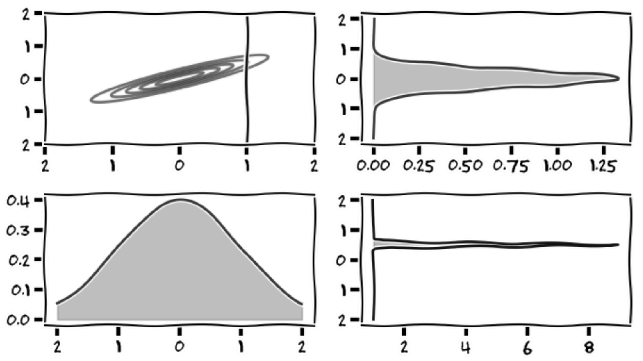
\includegraphics[scale=2]{img/probExamples.png}

\theorem{Product Rule}
For random variables $X$ \& $Y$
$$\prob(X=x,Y=Y)=\prob(Y=y|X=x)\prob(X=x)$$

\theorem{Sum Rule}
For random variables $X$ \& $Y$
$$\prob(X=x)=\sum_j\prob(X=x,Y=y_j)$$

\theorem{Baye's Theorem}
For random variables $X$ \& $Y$
$$\prob(X=x|Y=y)=\frac{\prob(Y=y|X=x)\prob(X=x)}{\prob(Y=y)}$$

\definition{Elements of Bayes' Theorem}
The elements of \textit{Bayes' Theory} can be broken down to explain parts of the model.
$$\underbrace{\prob(\theta|Y)}_{\text{Posterior}}=\frac{\overbrace{\prob(Y|\theta)}^{\text{Likelihood}}\overbrace{\prob(\theta)}^{\text{Prior}}}{\underbrace{\prob(Y)}_{\text{Evidence}}}$$
\begin{tabular}{l|l}
Posterior&Which parameters of the model do I belive produce distributions have generated the data $Y$\\
Likelihood&How likley is the data to come from the model specifely indexed by $\theta$\\
Prior&What distribution do I think parameter $\theta$ has\\
Evidence&How likely do I think data $Y$ is for all models.
\end{tabular}
\nb The \textit{Evidence} normalises this function.\\

\definition{Conjugate Prior}
If the \textit{Prior} is the same probability distribution family as the \textit{Posterior} then the \textit{Prior} is called a \textit{Conjugate Prior}.\\

\definition{Expectaction Value, $\expect$}
The mean value a random variable will produce from a large number of samples.\\
\begin{tabular}{l|l}
Continuous&Discrete\\\hline
$\expect(X)=\int_{-\infty}^{\infty} x\prob(X)dx$&$\expect(X)=\sum_{-\infty}^{\infty} x\prob(X)dx$\\
$\expect(f(X))=\int_{-\infty}^{\infty} f(x)\prob(X)dx$&$\expect(f(X))=\sum_{-\infty}^{\infty} f(x)\prob(X)dx$
\end{tabular}\\

\definition{Variance}
Describes the amount of spread in the values a single random variable will produce.
$$\var(X)=\expect\left(x-\expect(x))^2\right)=\expect(X^2)-\bigg(\expect(X)\bigg)^2$$

\definition{Covariance}
Describes the joint variability between two random variables.
$$\cov(X,Y)=\expect\bigg(\big(X-\expect(X)\big)\big(Y-\expect(Y)\big)\bigg)$$

\definition{Marginalisation}
The process of summing out the probability of one random variable using its joing probability with another rando variable.
\[\begin{array}{rrcl}
\mathrm{Continuous}&\prob(X=x)&=&\int(X=x,Y=y)dy\\
\mathrm{Discrete}&\prob(X=x)&=&\sum_i\prob(X=x,Y=y_i)
\end{array}\]

\definition{Likelihood Function}
Define $\X\sim f_n(\cdot;\theta^*)$ for some unknown $\theta^*\in\Theta$ and let $\x$ be an observation of $\X$.\\
A \textit{Likelihood Function} is any function, $L(\cdot;\x):\Theta\to[0,\infty)$, which is proportional to the PMF/PDF of the obeserved realisation $\x$.
$$L(\theta;\x):=Cf_b(\x;\theta)\ \forall\ C>0$$
\nb Sometimes this is called the \textit{Observed} Likelihood Function since it is dependent on observed data.\\

\definition{Log-Likelihood Function}
Let $\X\sim f_n(\cdot;\theta^*)$ for some unknown $\theta^*\in\Theta$ and $\x$ be an observation of $\X$.\\
The \textit{Log-Likelihood Function} is the natural log of a \textit{Likelihood Function}
$$\ell(\theta;\x):=\ln f_n(\x;\theta)+C,\ C\in\reals$$

\definition{Maximum Likelihood Estimation}
The \textit{Maximum Likelihood Estimate} is an estimate for a parameter of a probability distribution which is the value which maximises the \textit{Likelihood Function} (or the \textit{Likelihood Function}).
$$\hat{\theta}:=\text{argmax}_\theta L(\theta;\x)$$

\definition{Central Limit Theorem}
The distribution of the sum (or mean) of a large number of independent, identically distributied random variables can be approximated to a normal distribution, regardless of the distributions of the random variables.

\section{Distributions}

\definition{Bernoulli Distribution}
Models an event with a binary outcome (0 or 1) with parameter $p$ st $\prob(X=1)=p$
Let $X\sim\text{Bernoulli}(p)$. Then
\[\begin{array}{rcl}
f_X(x)&=&\begin{cases}
p&, x=1\\
1-p&, x=0\\
0&\text{otherwise}
\end{cases}\\
F_X(x)&=&\begin{cases}
0&,x<0\\
1-p&0\leq x<1\\
1&x\geq1
\end{cases}\\
\expect(X)&=&p\\
\text{Var}(X)&=&p(1-p)
\end{array}\]

\definition{$\beta$-Distribution}
A \textit{$\beta$-Distribution} is a continuous distribution over interval $[0,1]$ which is parameterised by two positive \textit{shape parameters}, $\alpha\ \&\ \beta$. A \textit{$\beta$-Distribution} can be used to encode assumptions as a \textit{Prior}.\\
Let $X\sim\beta(\alpha,\beta)$. Then
\[\begin{array}{rcl}
f_X(x)&=&\dfrac{\Gamma(\alpha+\beta)}{\Gamma(\alpha)+\Gamma(\beta)}x^{\alpha-1}(1-x)^{\beta-1}
\end{array}\]

\example{$\beta$-Distribution}
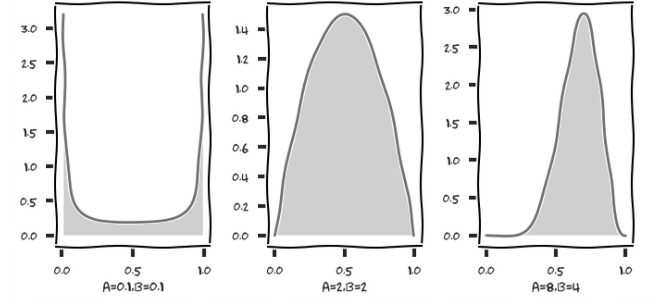
\includegraphics[scale=.6]{img/betaExamples.png}

\definition{Direchlet Distribution}
Let $X\sim\text{Dir}(\pmb{\alpha})$. Then
$$f_X(x):=\dfrac{\Gamma(\alpha_0)}{\Gamma(\alpha_1)\times\dots\times\Gamma(\alpha_N)}\prod_{i=1}^Nx_i^{\alpha_{i-1}}$$

\definition{Exponential Distribution Family}
The \textit{Exponential Distribution Family} is a set of probability distributions which fit the form.
$$\prob(\x|\pmb{\theta})=h(\x)g(\pmb{\theta})e^{\pmb{\theta}^T\textbf{u}(\x)}$$
With conjugate prior
$$\prob(\pmb{\theta}|\pmb{\chi},\nu)=f(\pmb{\chi},\nu)g(\pmb{\chi})^\nu e^{\nu\pmb{\theta}^T\pmb{\chi}}$$

\definition{Multivariate Normal Distribution}
Let $\X\sim\mathcal{N}(\mub,\pmb{\Sigma})$. Then
$$f_\X(\x)=\dfrac{1}{(2\pi)^{N/2}|\pmb{\Sigma}^{1/2}}e^{-\frac{1}{2}(\x-\mub)^T\pmb{\Sigma}^{-1}(\x-\mub)}$$
\nb Also known as \textit{Gaussian Distribution}.\\

\remark{Conjugate Prior for Normal Distribution}
For a \textit{Normal Distribution} the conjugate prior of $\mub$ is \textit{Gaussian} and the conjugate prior of $\pmb{\Sigma}$ is \textit{Inverse-Wishard}.\\

%TODO - Study conjugacy

\newpage
\setcounter{section}{-1}
\section{Appendix}

\proof{Deriving Gaussian Marginal Distribution}
\textit{NOTE - This is dense as fuck \& uses quite a bit of bullshit}.\\
\\Let $\X\sim\mathcal{N}\left(\begin{pmatrix}
\mub_1\\\mub_2
\end{pmatrix},\begin{pmatrix}
\Lambda_{11}&\Lambda_{12}\\
\Lambda_{21}&\Lambda_{22}
\end{pmatrix}^{-1}\right)$.\\
$\mub_1,\mub_2$ can be considered as two parts of the mean vector $\mub$.\\
Let $\x$ be a realisation of $\X$ where $\x:=(\x_1,\x_2)$ with $\x_1\ \&\ \x_2$ representing the same partition as $\mub_1\ \&\ \mub_2$ respecitvely.\\
Define $D:=\mathrm{dim}(\x),\ D_1:=\mathrm{dim}(\x_1)\ \&\ D_2:=\mathrm{dim}(\x_2)$.\\
\\Here we want to get from $\prob(\x_1,\x_2)$ to $\prob(\x_1)$.\\
Consider the exponent of the joint distribution
$$E=-\frac{1}{2}(\x_1-\mub_1)^T\Lambda_11(\x_1-\mub_1)-\frac{1}{2}(\x_1-\mub_1)^T\Lambda_{12}(\x_2-\mub_2)-\frac{1}{2}(\x_2-\mub_2)^T\Lambda_{21}(\x_1-\mub_1)-\frac{1}{2}(\x_2-\mub_2)^T\Lambda_{22}(\x_2-\mub_2)$$
To produce the marginal for $x_1$ we want to isolate the terms involving $x_2$ so they are easy to remove.
\[\begin{array}{rcl}
E&=&-\frac{1}{2}\bigg[\left(\x_2^T\Lambda_{22}\x_2-2\x_2^T\Lambda_22(\mub_2-\Lambda_{22}^{-1}\Lambda_{21}(\x_1-\mub_1))\right)\\
&-&2\x_1^T\Lambda_{12}\mub_2+2\mub_1^T\Lambda_{12}\mub_2+\mub_2^T\Lambda_{22}\mub_2+\x_1^T\Lambda_{11}\x_1\\
&-&2\x_1^T\Lambda_11\mub_1+\mub_1^T\Lambda_{11}\mub_1\bigg]\\
&=&\underbrace{-\frac{1}{2}\left(\x_2-(\mub_2-\Lambda_{22}^{-1}\Lambda_{21}(\x_1-\mub_1))\right)^T\Lambda_{22}\left(\x_2-(\mub_2-\Lambda_{22}^{-1}\Lambda_{21}(\x_1-\mub_1))\right)}_{E_1}\\
&+&\underbrace{\frac{1}{2}\left(\x_1^T\Lambda_{12}\Lambda_{22}^{-1}\Lambda_{21}\x_1-2\x_1^T\Lambda_{12}\Lambda_{22}^{-1}\Lambda_{21}\mub_1+\mub_1^T\Lambda_{12}\Lambda_{22}^{-1}\Lambda_{21}\mub_1\right)}_{A}\\
&-&\underbrace{\frac{1}{2}\left(\x_1^T\Lambda_11\x_1-2\x_1^T\Lambda_{11}\mub_1+\mub_{1}\Lambda_{11}\mub_1\right)}_{B}
\end{array}\]
Note that $A$ \& $B$ do not contain any $x_2$ terms.\\
Since the co-variance matrix is symmetric we have $\Lambda_{12}=\Lambda_{21}^T$ we have
$$\x_1^T\Lambda_{12}\mub_2=\x_1^T\Lambda_{21}^T\mub_2=(\Lambda_{21}\x_1)^T\mub_2=\mub_2^T\Lambda_{21}\x_1$$
We shall not rewrite $A$ \& $B$ as quadratic expressions
\[\begin{array}{rrcl}
&A&=&\dfrac{1}{2}\left(\x_1^T\Lambda_{12}\Lambda_{22}^{-1}\Lambda_{21}\x_1-2\x_1^T\Lambda_{12}\Lambda_{22}^{-1}\Lambda_{21}\mub_1+\mub_1^T\Lambda_{12}\Lambda_{22}^{-1}\Lambda_{21}\mub_1\right)\\
&&=&\dfrac{1}{2}(\x_1-\mub_1)^T(\Lambda_{12}\Lambda_{22}^{-1}\Lambda_{21})(\x_1-\mub_1)\\
&B&=&\dfrac{1}{2}\left(\x_1^T\Lambda_{11}\x_1-2\x_1^T\Lambda_{11}\mub_1+\mub_{1}\Lambda_{11}\mub_1\right)\\
&&=&\dfrac{1}{2}(\x_1-\mub_1)^T\Lambda_{11}(\x_1-\mub_1)\\
\implies&A-B&=&\frac{1}{2}(\x_1-\mub_1)^T(\Lambda_{12}\Lambda_{22}^{-1}\Lambda_{21}-\Lambda_{11})(\x_1-\mub_1)\\
&\mathrm{Let\ }E_2&:=&A-B
\end{array}\]
Now the exponent has been orgainised we can consider the whole gaussian expression.
\[\begin{array}{rcll}
\prob(\x_1,\x_2)&=&\dfrac{e^{E_1}e^{E_2}}{(2\pi)^{\frac{D}{2}}|\Sigma|^{\frac{1}{2}}}\\
\prob(\x_1)&=&{\displaystyle\int\prob(\x_1,\x_2)d\x_2}\\
&=&{\displaystyle\int\dfrac{e^{E_1}e^{E_2}}{(2\pi)^{\frac{D}{2}}|\Sigma|^{\frac{1}{2}}}d\x_2}\\
&=&{\dfrac{e^{E_2}}{(2\pi)^{\frac{D}{2}}|\Sigma|^{\frac{1}{2}}}\displaystyle\int e^{E_1}d\x_2}&\text{Since $E_2$ is independent of $\x_2$}
\end{array}\]
Now we consider $\int e^{E_1}d\x_2$.\\
Since we know a gaussian must intergrate to 1 over the whole domain we deduce that
\[\begin{array}{rrcl}
&{\displaystyle\int\dfrac{1}{(2\pi)^{\frac{D_2}{2}}|\Lambda_{22}^{-1}|^{\frac{1}{2}}}e^{E_1}d_{\x_2}}&=&1\\\
\implies&\int e^{E_1}d\x_2&=&(2\pi)^{\frac{D_2}{2}}|\Lambda_{22}^{-1}|^{\frac{1}{2}}
\end{array}\]
\nb $\Lambda_{22}^{-1}$ is the variance of $\x_2$.\\
Using the result of this intergal we have
\[\begin{array}{rcl}
\prob(\x_1)&=&(2\pi)^{\frac{D_2}{2}}|\Lambda_{22}^{-1}|^{\frac{1}{2}}\dfrac{1}{(2\pi)^{\frac{D}{2}}|\Sigma|^{\frac{1}{2}}}e^{E_2}\\
&=&\dfrac{e^{E_2}}{(2\pi)^{\frac{D-D_2}{2}}|\Lambda_{22}^{-1}|^{-\frac{1}{2}}|\Sigma|^{\frac{1}{2}}}
\end{array}\]
The Schur complement of $\Lambda_{22}$ is $\Lambda^{-1}_{22}=\Sigma_{22}-\Sigma_{21}\Sigma_{11}^{-1}\Sigma_{12}$.\\
Thus \[\begin{array}{rcl}
|\Lambda_{22}^{-1}|^{-\frac{1}{2}}|\Sigma|^{\frac{1}{2}}&=&|\Sigma_{22}-\Sigma_{21}\Sigma_{11}^{-1}\Sigma_{12}|^{-\frac{1}{2}}|\Sigma_{11}|^{\frac{1}{2}}|\Sigma_{22}-\Sigma_{21}\Sigma_{11}^{-1}\Sigma_{12}|^{\frac{1}{2}}\\
&=&|\Sigma_{11}|^{\frac{1}{2}}
\end{array}\]
Now we have a full expression
\[\begin{array}{rcl}
\prob(\x_1)&=&\dfrac{e^{E_2}}{(2\pi)^{\frac{D-D_2}{2}}|\Lambda_{22}^{-1}|^{-\frac{1}{2}}|\Sigma|^{\frac{1}{2}}}\\
&=&\dfrac{1}{(2\pi)^{\frac{D_1}{2}}|\Sigma_{11}|^{\frac{1}{2}}}e^{-\frac{1}{2}(\x_1-\mub_1)^T\Sigma_{11}^{-1}(\x_1-\mub_1)}
\end{array}\]
$\hfill{\blacksquare}$

\proof{Deriving Gaussian Conditional Distribution}
\\Let $\X\sim\mathcal{N}\left(\begin{pmatrix}
\mub_1\\\mub_2
\end{pmatrix},\begin{pmatrix}
\Sigma_{11}&\Sigma_{12}\\
\Sigma_{21}&\Sigma_{22}
\end{pmatrix}\right)$.\\
$\mub_1,\mub_2$ can be considered as two parts of the mean vector $\mub$.\\
Let $\x$ be a realisation of $\X$ where $\x:=(\x_1,\x_2)$ with $\x_1\ \&\ \x_2$ representing the same partition as $\mub_1\ \&\ \mub_2$ respecitvely.\\
Define $D:=\mathrm{dim}(\x)$.\\
\\We want to find the distribution of $\prob(\x_1|\x_2)$.\\
From the product rule we know that $\prob(\x_1,\x_2)=\prob(\x_1|\x_2)\prob(\x_2)$ and we already know the joint \& marginal distributions for a gaussian.\\
We have that
$$
\prob(\x_1,\x_2)\propto e^{-\frac{1}{2}\begin{pmatrix}
\x_1-\mub_1\\\x_2-\mub_2
\end{pmatrix}^T\begin{pmatrix}
\Sigma_{11}&\Sigma_{12}\\
\Sigma_{21}&\Sigma_{22}
\end{pmatrix}^{-1}\begin{pmatrix}
\x_1-\mub_1\\\x_2-\mub_2
\end{pmatrix}}$$
We now want to factor the marginal distribution out of this expression.
$$
\prob(\x_2)\propto e^{-\frac{1}{2}(\x_2-\mub_2)^T\Sigma_{22}^{-1}(\x_2-\mub_2)}
$$
Lets look at the exponent of the joint distribution.\\
\nb About to use a lot of Schur Complements
\[\begin{array}{rl}
E&=-\dfrac{1}{2}\begin{pmatrix}
\x_1-\mub_1\\\x_2-\mub_2
\end{pmatrix}^T\begin{pmatrix}
\Sigma_{11}&\Sigma_{12}\\
\Sigma_{21}&\Sigma_{22}
\end{pmatrix}^{-1}\begin{pmatrix}
\x_1-\mub_1\\\x_2-\mub_2
\end{pmatrix}\\
&=-\dfrac{1}{2}\begin{pmatrix}
\x_1-\mub_1\\
\x_2-\mub_2
\end{pmatrix}^T
\begin{pmatrix}
I&0\\
\Sigma_{22}^{-1}\Sigma_{21}&I
\end{pmatrix}^T
\begin{pmatrix}
(\Sigma/\Sigma_{22})^{-1}&0\\
0&\Sigma_{22}^{-1}
\end{pmatrix}
\begin{pmatrix}
I&-\Sigma_{12}\Sigma_{22}^{-1}\\
0&I
\end{pmatrix}
\begin{pmatrix}
\x_1-\mub_1\\
\x_2-\mub_2
\end{pmatrix}\\
&=-\dfrac{1}{2}\begin{pmatrix}
\x_1-\mub_1\\
\x_2-\mub_2
\end{pmatrix}^T
\begin{pmatrix}
(\Sigma/\Sigma_{22})^{-1}&-(\Sigma/\Sigma_{22})^{-1}\Sigma_{12}\Sigma_{22}^{-1}\\
-\Sigma_{21}\Sigma_{22}^{-1}(\Sigma/\Sigma_{22})^{-1}&\Sigma_{22}^{-1}
\end{pmatrix}^{-1}
\begin{pmatrix}
\x_1-\mub_1\\
\x_2-\mub_2
\end{pmatrix}\\
&=-\dfrac{1}{2}\bigg[\x_1-(\mub_1+\Sigma_{21}\Sigma_{22}^{-1}(\x_2-\mub_2))\bigg]^T(\Sigma/\Sigma_{22})^{-1}\bigg[\x_1-(\mub_1+\Sigma_{21}\Sigma_{22}^{-1}(\x_2-\mub_2))\bigg]\\
&\underbrace{-\dfrac{1}{2}(\x_2-\mub_2)^T\Sigma_{22}^{-1}(\x_2-\mub_2)}_{E_2}
\end{array}\]
Note that $E_2$ is exactly the exponent for the marginal distribution of $\x_2$ and thus what we want to factory out in order to get to the conditional distribution.
$$\prob(\x_1|\x_2)\propto e^{-\dfrac{1}{2}\big[\x_1-\underbrace{(\mub_1+\Sigma_{21}\Sigma_{22}^{-1}(\x_2-\mub_2))}_{\text{mean}}\big]^T(\underbrace{\Sigma/\Sigma_{22}}_{\text{covariance}})^{-1}\big[\x_1-(\mub_1+\Sigma_{21}\Sigma_{22}^{-1}(\x_2-\mub_2))\big]}$$
$\hfill{\blacksquare}$

\end{document}
